%! suppress = Unicode
%! Author = breandan
%! Date = 11/16/20

% Preamble
\documentclass[11pt]{article}

% Packages
\usepackage{amsmath}
\usepackage[pdf]{graphviz}
\usepackage{amssymb}
\usepackage{mathrsfs}

\newcommand*\circled[1]{\tikz[baseline=-0.1cm]{
    \node[shape=circle,draw,inner sep=0.5pt] (char) {\fontsize{7}{12}\textsf{#1}};}}

\usepackage{unicode-math}
\DeclareMathAlphabet{\mathcal}{OMS}{cmsy}{m}{n}
\usepackage{cancel}
\newcommand{\nDownarrow}{\ensuremath{\text{ }\cancel{\Downarrow}\text{ }}}
\usepackage{centernot}

\usepackage{pgfplots}
\usepgfplotslibrary{fillbetween}
\usetikzlibrary{patterns}
\pgfmathdeclarefunction{gauss}{2}{%
\pgfmathparse{1/(#2*sqrt(2*pi))*exp(-((x-#1)^2)/(2*#2^2))}%
}

\usepackage{arydshln}
\usepackage{adjustbox}
\usepackage{enumerate}
\usepackage{enumitem}
\usepackage{tikz-cd}
\usetikzlibrary{calc}
\usepackage{amsfonts}
%\usepackage{prooftrees}
\usepackage{bussproofs}
\usepackage{hyperref}
\renewcommand{\sectionautorefname}{\S}
\renewcommand{\subsectionautorefname}{\S}
\usepackage{natbib}
\usepackage{float}
\usepackage{xcolor}

\usepackage{tikz-3dplot}
\usetikzlibrary{3d}
\usetikzlibrary{calligraphy}
\newif\ifshowcellnumber
\showcellnumbertrue

\usepackage{algpseudocode}
\usepackage{algorithmicx}
\usepackage{sourcecodepro}
\usepackage{listings}
\usepackage{tikz-qtree}
\usepackage{amsthm}
\usepackage{bm}
\usetikzlibrary{bayesnet}
\usetikzlibrary{arrows}
\usepackage{caption}
\usepackage{subcaption}
\usetikzlibrary{backgrounds}

\newcommand{\E}{\mathbb{E}}
\newcommand{\Var}{\mathrm{Var}}
\newcommand{\Cov}{\mathrm{Cov}}

\newcommand{\CompOrder}{\mathcal{O}}
\def\graphspace{\mathbf{G}}
\def\Uniform{\mbox{\rm Uniform}}
\def\Gaussian{\mbox{\rm Gaussian}}
\def\Bernoulli{\mbox{\rm Bernoulli}}
\def\Dirichlet{\mbox{\rm Dirichlet}}

\usepackage{mathtools}% superior to amsmath
\usepackage{tikz}
\usepackage{graphicx}


\title{Pattern Recognition in Procedural Knowledge}
\author{Breandan Considine}
\date{\today}

% Document
\begin{document}
    \maketitle

    \tableofcontents
    \pagebreak


    \section{Introduction}

    Historically, most knowledge was stored as natural language. A growing portion is now \textit{code}~\citep{allamanis2018survey}. The majority of code is procedural knowledge, written by a human and intended to operate a machine. Though it shares many statistical properties in common with natural language~\citep{hindle2012naturalness}, code has an unambiguous grammar and well-defined semantics~\citep{pierce2010software}. We can use these properties to precisely reason about operational or procedural correctness.

    Prior work explored differentiable programming~\citep{considine2019programming}. Differentiability plays a key role in learning, but does not provide the necessary vocabulary to describe human knowledge. In order to capture human knowledge and begin to reason as humans do, programs must be able to express the concept of \textit{uncertainty}. We propose a set of tools and techniques for reasoning about uncertainty in the form of \textit{procedural knowledge}. In our work, we define procedural knowledge as a graph whose topology represents how to structure computation in order to achieve some desired programming task.

    To reason about procedural knowledge, we must first define what it means for two procedures to be equal. Although equality is known to be undecidable in most languages, various equivalence tests and semi-decision procedures have been developed. For example, we could rewrite said procedures~\citep{baader1999term}, compare them in various contexts~\citep{felleisen1990expressive}, and simulate or execute them on various input data~\citep{chen2020metamorphic} so as to ascertain their exact relationship.

    In practice, exact equality is too rigid to operationalize. A more useful theory would allow us to compare two similar procedures in the presence of naturally-arising stochasticity. What is the probability of observing local variations? How are those observations related? And how do local variations affect global behavior? In order to correctly pose these questions and begin to answer them, we must be able to reason probabilistically.

    Graphs are a natural representation for both procedural knowledge~\citep{allamanis2017learning} and probabilistic reasoning~\citep{pearl2014probabilistic}, both enabling a large class of useful data transformations and vastly simplifying their implementation on physical machinery. Depending on the author's perspective, it is possible to view the evaluation of these routines as either operating a stateful machine, reducing a symbolic expression or running a dynamical process on a dataflow graph.

    In this work, we first  define exact and approximate equality and cover some deterministic and probabilistic algorithms for deciding it (\S~\ref{sec:definitions}). We then describe a few graph representations for encoding approximate procedural knowledge (\S~\ref{sec:graphs}). Finally, we will discuss some opportunities for applying these ideas to search-based software engineering, in particular, documentation alignment, code search, synthesis and DSL generation (\S~\ref{sec:applications}).


    \section{From exact to approximate equality}\label{sec:definitions}

    Reason is the source of all human knowledge. In order to understand reason, we need to understand how concepts are related. Next to identity, one of the simplest relations is equality. Equality is like identity for objects that may differ in superficial ways, but are the same in all but name and appearance.

    For such a fundamental concept, the notation for equality is recklessly overloaded in mathematics and computer science. Depending on context, $x = y$ may denote: (1)~define $x$ to be $y$, (2)~$x$ and $y$ are the same, (3)~are $x$ and $y$ the same? (4)~$x$ and $y$ are exchangeable, (5)~assign $y$ to $x$, (6)~assign $x$ to $y$, among other peculiar programming idioms. If two expressions are equal, it should be possible to treat them in the same manner.

    But this convention does not always hold! Suppose we need to compute the derivative of a logical function with respect to its inputs. The trouble is, logical equality is not differentiable. Consider the Kronecker $δ$-function:

    $$
    δ_k(x, y) :=
    \begin{cases}
        1 \text{ if } x \overset{?}{=} y, \\
        0 \text{ otherwise }\\
    \end{cases}
    $$

    When encountering $δ_k$, how should we represent its derivative? Since $\mathbb{B}$ is finite, $δ_k^{-1}(B\subset \mathbb{B})$ is not open, thus $δ_k$ is not continuous and $\nablaδ_k$ is undefined. Now consider the Dirac $δ$-function, which is defined as follows:

    $$
    \forall f \in \mathbb{R}^2 \rightarrow \mathbb{R}, \int_{\mathbb{R}^2} f(x,y)δ_d(x-a,y-b)d(x, y) \overset{Δ}{=} f(a,b)
    $$

    Unlike $\nablaδ_k$, it can be shown that $\nablaδ_d$ is well-behaved everywhere on $\mathbb{R}^2$. However we encounter an important distinction between intensional and extensional equality. Unlike elementary functions, there exist many functions which can only be described indirectly, e.g. a probability distribution on a set of measure zero. Nevertheless, these constructions are convenient abstractions for modeling many physical and computational processes.

    Neither $δ_k$ nor $\nablaδ_d$ are a satisfactory basis for logical equality. To allow a more flexible definition of the $\overset{?}{=}$ operator, we require a relation which approximates the logical properties of $δ_k$, but can be made differentiable like $δ_d$. A more general notion is the concept of an \textit{equivalence relation} $\equiv$, a binary relation with the following logical properties:

    \begin{prooftree}
        \bottomAlignProof
        \AxiomC{}
        \UnaryInfC{$a \equiv a$\vphantom{$()$}}
        \noLine
        \UnaryInfC{}
        \noLine
        \UnaryInfC{\textit{Identity}}
        \DisplayProof
        \hskip 1.5em
        \bottomAlignProof
        \AxiomC{$a \equiv b$}
        \UnaryInfC{$b \equiv a$\vphantom{$()$}}
        \noLine
        \UnaryInfC{}
        \noLine
        \UnaryInfC{\textit{Symmetry}}
        \DisplayProof
        \hskip 1.5em
        \bottomAlignProof
        \AxiomC{$a \equiv b$}
        \AxiomC{$b \equiv c$}
        \BinaryInfC{$a \equiv c$\vphantom{$()$}}
        \noLine
        \UnaryInfC{}
        \noLine
        \UnaryInfC{\textit{Transitivity}}
        \DisplayProof
        \hskip 1.5em
        \bottomAlignProof
        \AxiomC{$a \equiv b$}
        \UnaryInfC{$f(a) \equiv f(b)$}
        \noLine
        \UnaryInfC{}
        \noLine
        \UnaryInfC{\textit{Congruence}}
    \end{prooftree}

    \pagebreak\subsection{Decidability}\label{sec:algorithms}

    To determine if two procedures are equal, we need a decision procedure. We list several high-level approaches for deciding exact and approximate equality in the deterministic and probabilistic setting in the table below:

    \bgroup
    \def\arraystretch{1.2}
    \begin{table}[H]
        \centering
        \begin{tabular}{c|l:l}
            & \textbf{Deterministic} & \textbf{Probabilistic} \\ \hline
            \multicolumn{1}{c|}{\textbf{Exact}} & \begin{tabular}[c]{@{}l@{}}
                                                       Type Checking\\ Model Checking
            \end{tabular} & \begin{tabular}[c]{@{}l@{}}
                                Variable Elimination\\Probabilistic Circuits
            \end{tabular} \\\hdashline
            \multicolumn{1}{c|}{\textbf{Approximate}} & \begin{tabular}[c]{@{}l@{}}
                                                             Software Testing\\Dynamic Analysis
            \end{tabular} & \begin{tabular}[c]{@{}l@{}}
                                Monte Carlo Methods\\Bayesian Networks
            \end{tabular}
        \end{tabular}
    \end{table}
    \egroup

    It is seldom the case that two semantically equal expressions are trivially equal: we must first perform some computation to establish their equality. In the exact setting, this procedure might be summarized as follows:

    \begin{enumerate}
        \item Rewrite: Either enumerate a set of equivalent expressions, or reduce the proposition into normal form if possible, then,
        \item Compare: Perform a computationally trivial (e.g. $\mathcal{O}(n)$) comparison.
    \end{enumerate}

    Unfortunately, exact equality is known to be undecidable in first~\cite{godel1929vollstandigkeit} and higher order theories~\cite{godel1931formal}. We know there can be no machine which accepts every equality and rejects every disequality in a universal language~\cite{turing1937computable}. By extension, any nontrivial property of partial functions is undecidable~\cite{rice1953classes}.

    Tractability may be related to, but is not contingent upon decidability. When decidable, equality may be intractable in practice, and languages where equality is undecidable may have decidable fragments. But even when exact equality is intractable, we may be able to construct a probabilistic decision procedure (PDP) or semidecision procedure (SDP) terminating for all practical purposes. The latter approaches fall into two broad categories:

    \begin{itemize}
        \item Execute: Evaluate the program by running it on a small set of inputs
        \item Sample: Build a probabilistic model and sample from its distribution
    \end{itemize}

    In the following section, we will introduce a few compatible theories corresponding to intensional and extensional equality, then build on those definitions to include recent approaches to exact and approximate equality in the determinsitic and probabilistic setting. In so doing, we will see there is a delicate tradeoff between complexity, sensitivity and specificity.

    \subsection{Intensional equivalence}\label{subsec:in-eq}

    Let $Ω \subseteq \mathcal{F} \times \mathcal{F}$ be a relation on representable functions which are closed under composition. We say two representations $f, g \in \mathcal{X} \rightarrow \mathcal{Y}$ are intensionally equal under $Ω$ if we can establish that $g \in Ω^n(f)$ for some $n \in \mathbb{N}$.

    \begin{prooftree}
        \AxiomC{$f, g: \mathcal{X \rightarrow Y} \in Γ^0_{g}$}
        \RightLabel{\textsc{Init}}
        \UnaryInfC{$Γ^0_{g} \vdash \{f\}, \{(f, f)\}$}
%        \UnaryInfC{\textit{Commutivity}}
        \DisplayProof
        \hskip 1em
        \AxiomC{$Γ^{n}_{g} \vdash E \subseteq \mathcal{F}, G \subseteq E \times E$}
        \RightLabel{\textsc{Sub}}
        \UnaryInfC{$Γ^{n+1}_{g} \vdash \bigcup\limits_{\substack{e \in E\\\sigma \in Ω}}e'\leftarrow e[\sigma_1\rightarrow\sigma_2], (e, e')$}
        \DisplayProof
        \vskip 1em
        \AxiomC{$Γ^n_{g} \vdash E, G$}
        \AxiomC{$g \in E$}
        \RightLabel{\textsc{Eq}}
        \BinaryInfC{$Γ^n_{g} \vdash f \equiv_Ω g$ by $G^{-n}(g)$}
        \DisplayProof
        \hskip 1em
        \AxiomC{$Γ^n_{g} \vdash E$}
        \AxiomC{$Γ^{n+1}_{g}\vdash E$}
        \AxiomC{$g\notin E$}
        \RightLabel{\textsc{Neq}}
        \TrinaryInfC{$Γ^{n+1}_{g} \vdash f \not\equiv_Ω g$}
    \end{prooftree}

    \noindent For example, suppose we are given $f: \{a, b, c\} \mapsto a b c, g: \{a, b, c\} \mapsto c b a$ and $Ω := \{(a, a), (ab, ba)\}$. Indeed, $\textsc{Eq}[f, g]$ can be established as follows:

    \vspace{-10pt}\begin{prooftree}
        \def\fCenter{\ := \ }
        \Axiom$f \fCenter abc, \text{ } g := cba \in Γ_g^0$
        \def\fCenter{\ \vdash\ }
        \RightLabel{\textsc{Init}}
        \UnaryInf$Γ^0_{g} \fCenter \{abc\}, \{(abc, abc)\}$
        \RightLabel{\textsc{Sub}}
        \UnaryInf$Γ^1_{g} \fCenter \{\ldots, bac, acb\}, \{\ldots, (abc, bac), (abc, acb)\}$
        \RightLabel{\textsc{Sub}}
        \UnaryInf$Γ^2_{g} \fCenter \{\ldots, bca, cab\}, \{\ldots, (bac, bac), (acb, acb), (bac, bca), (acb, cab)\}$
        \RightLabel{\textsc{Sub}}
        \UnaryInf$Γ^3_{g} \fCenter \{\ldots, \mathbf{cba}\}, \{\ldots, (bca, bca), (cab, cab), (cab,\textbf{cba})\}$
        \RightLabel{\textsc{Eq}}
        \UnaryInf$Γ^3_{g} \fCenter f \equiv_Ω g\text{ by } G^{-3}(g:=cba) = \{f := abc\}$
    \end{prooftree}

    \noindent We can visualize $G$ as a directed graph, omitting all loops. Notice how each path converges to the same term, a property known as $\textit{strong confluence}$.

    \hspace{12pt}\digraph[scale=0.5]{abcint}{
    node[ fontname="CMU Classical Serif" fontsize=20 shape=Mrecord ];
    edge[ fontname="CMU Classical Serif" fontsize=18 ];
    rankdir=LR;
    len=3;

    a [ label="abc"; ]
    b [ label="bac"; ]
    c [ label="acb"; ]
    d [ label="bca"; ]
    e [ label="cab"; ]
    f [ label="cba"; ]

%    a -> a [label="Σ₀"]
    a -> b [label=<Ω<SUB>2</SUB>> minlen=2]
    a -> c [label=<Ω<SUB>2</SUB>> minlen=2]
    b -> d [label=<Ω<SUB>2</SUB>> minlen=2]
    c -> e [label=<Ω<SUB>2</SUB>> minlen=2]
    e -> f [label=<Ω<SUB>2</SUB>> minlen=2]
    d -> f [label=<Ω<SUB>2</SUB>> minlen=2]
    }

    \noindent Let us suppose $|\mathcal{X}|, |Ω^*| \in \mathbb{N}$ and consider the complexity of establishing $\textsc{Eq}[f, g], \forall f \equiv_Ω g \in \mathcal{X} \rightarrow \mathcal{Y}$. It can be shown the above procedure requires:

    $$\mathcal{O}_{\textsc{Eq}} = \underset{i \leq n}{\text{max }}\underset{n}{\text{argmin}}\{|G| \mid Γ^i_{g} \vdash G, Γ_{g}^n = Γ_{g}^{n+1}\}$$ % \text{, or } \Theta_{\textsc{Eq}}(|\mathcal{X}|!) \text{ for } Ω.$$

    \noindent Assuming termination, $\mathcal{O}_{\textsc{Eq}} = \Theta_{\textsc{Neq}}$ although $\mathbb{E}[\Theta_\textsc{Eq}|f \equiv g]$ is more tractable. However termination is not necessarily guaranteed, e.g. $Ω' := \{(a, 1a)\}$. Equality and termination under arbitrary $Ω$ are known to be undecidable~\citep{baader1999term}.

    \subsection{Computational equivalence}\label{subsec:comp-eq}

    Clearly, the procedure defined in \S~\ref{subsec:in-eq} is highly sensitive to $|\mathcal{X}|$ and $Ω$. While equality may be tractable, disequality is definitely an obstacle. In the computational setting, we will see the opposite holds, ceteris paribus. %Two values $r, r': \mathcal{Y}$ share a normal form in which equality is trivial.

    \begin{prooftree}
        \AxiomC{$fg: \mathcal{X} \rightarrow \mathcal{Y}, Ω: \{\mathcal{X}\rightarrow \mathcal{Y}\}\rightarrow \mathcal{Y} \in Γ$}
        \RightLabel{\textsc{Inv}}
        \UnaryInfC{$Γ \vdash fg(Ω) \Downarrow f(Ω) \cdot g(Ω)$}
        \DisplayProof
        \hskip 1em
        \AxiomC{$Γ \vdash f$}
        \AxiomC{$Γ \vdash Ω$}
        \RightLabel{\textsc{Sub}}
%        \AxiomC{$i: \mathcal{X}$}
        \BinaryInfC{$Γ \vdash f(Ω) \Downarrow Ω[f]$}
        \DisplayProof
        \vskip 1em
        \AxiomC{$Γ, Γ' \vdash f(Ω) \Downarrow g(Ω) \text{ } \forall Ω$}
        \RightLabel{\textsc{Eq}}
        \UnaryInfC{$Γ, Γ' \vdash f \equiv g$}
        \DisplayProof
        \hskip 1em
        \AxiomC{$Γ, Γ' \vdash \exists Ω \mid f(Ω) \nDownarrow g(Ω) $}
        \RightLabel{\textsc{Neq}}
        \UnaryInfC{$Γ, Γ' \vdash f \not\equiv g$ by $Ω$}
    \end{prooftree}

    % big step semantics
%    Extensional equality asks``Do $f_1$ and $f_2$ behave in the same way over all inputs?''
    \noindent \textsc{Sub} loosely corresponds to $\eta$-reduction in the untyped $\lambda$-calculus, however $f \notin Ω$ is disallowed and we assume all variables are bound by \textsc{Inv}. Let us consider $f: \{a, b, c\}\mapsto abc, g: \{a, b, c\} \mapsto ac$ under $Ω:=\{(a, 1), (b, 2), (c, 2)\}$:

    %If we test $\hat i \in {-2, -1, 0, 1, \ldots}$, we have $f_1(-2)=f_2(-2)$, $f_1(-1)=f_2(-1)$, $f_1(0)=f_2(0)$, $f_1(1) \neq f_2(1)$. Once we detect an $f_1(\hat i) \neq f_2(\hat i)$, we can halt immediately.

    \vspace{-10pt}\begin{prooftree}
        \def\fCenter{\ :=}
        \def\defaultHypSeparation{\hskip -1.1in}
        \Axiom$f\fCenter abc, Ω:=\{(a, 1), (b, 2), (c, 2)\} \in Γ$
        \def\fCenter{\ \vdash\ }
        \RightLabel{\textsc{Inv}}
        \UnaryInf$Γ \fCenter a(Ω)\cdot bc(Ω)$
        \RightLabel{\textsc{Sub}}
        \UnaryInf$Γ \fCenter 1\cdot bc(Ω)$
        \RightLabel{\textsc{Inv}}
        \UnaryInf$Γ \fCenter 1\cdot b(Ω)\cdot c(Ω)$
        \RightLabel{\textsc{Sub}}
        \UnaryInf$Γ \fCenter 2\cdot c(Ω)$
        \RightLabel{\textsc{Sub}}
        \UnaryInf$Γ \fCenter f(Ω) \Downarrow 4$
        \def\fCenter{\ :=}
        \Axiom$g\fCenter ac, Ω:=\{(a, 1), (b, 2), (c, 2)\} \in Γ'$
        \def\fCenter{\ \vdash\ }
        \RightLabel{\textsc{Inv}}
        \UnaryInf$Γ' \fCenter a(Ω)\cdot c(Ω)$
        \RightLabel{\textsc{Sub}}
        \UnaryInf$Γ' \fCenter 1\cdot c(Ω)$
        \RightLabel{\textsc{Sub}}
        \UnaryInf$Γ' \fCenter g(Ω) \Downarrow 2$
        \RightLabel{\textsc{Neq}}
        \BinaryInfC{$Γ, Γ' \vdash f \not\equiv g$ by $Ω :=\{(a, 1), (b, 2), (c, 2)\}$}
    \end{prooftree}

    \noindent We can view the above process as acting on a dataflow graph, where \textsc{Inv} backpropagates $Ω$, and \textsc{Sub} returns concrete values $\mathcal{Y}$, here depicted on $g$:

    \hspace{-30pt}\digraph[scale=0.5]{abcext0}{
    node[ fontname="CMU Classical Serif" fontsize=20 shape=Mrecord ];
    edge[ fontname="CMU Classical Serif" fontsize=18 ];
    rankdir=LR;
    len=3;

    f [ label="g"; ]
    a [ label="a"; ]
    c [ label="c"; ]
    d [ label="·"; ]

%    a -> a [label="Σ₀"]
    f -> d [label="Ω"]
    d -> a [label="Ω"]
    d -> c [label="Ω"]
    }\hspace{-20pt}\digraph[scale=0.5]{abcext1}{
    node[ fontname="CMU Classical Serif" fontsize=20 shape=Mrecord ];
    edge[ fontname="CMU Classical Serif" fontsize=18 ];
    rankdir=LR;
    len=3;

    f [ label="g"; ]
    a [ label="a"; ]
    c [ label="c"; ]
    d [ label="·"; ]

%    a -> a [label="Σ₀"]
    d -> f [label="𝓨"]
    a -> d [label="𝓨"]
    c -> d [label="𝓨"]
    }

    \noindent Assuming $f, g \sim P(\mathcal{F}), Ω \overset{iid}{\sim} P_\textsc{Test}(Ω \mid f \not\equiv g)$ yields a fixed but unknown distribution, $P_\textsc{Neq}(Ω) = P(f(Ω) \nDownarrow g(Ω) \mid f \not\equiv g)$. Let $\Theta_\textsc{Inv} = 1$ for all $f, Ω$. The complexity of certifying $\textsc{Neq}$ in $n$ trials follows a geometric distribution:

    \vspace{-10pt}$$\Theta_\textsc{Neq} \sim (1 - P_\textsc{Neq}(Ω))^nP_\textsc{Neq}(Ω) \text{ with } \mathop{\mathbb{E}}[\Theta_\textsc{Neq}] = (1-P_\textsc{Neq}(Ω))P_\textsc{Neq}(Ω)^{-1}$$

    \noindent Although a single witness $Ω$ s.t. $f(Ω) \nDownarrow g(Ω)$ is sufficient for disequality, this procedure may be intractable depending on $|\mathcal{X}|, P_\textsc{Neq}(Ω)$ and $\Theta_{\textsc{Inv}}$. Other fuzzing methods for selecting $Ω$ based on the structure of $f$ are also possible.

%    We can test using property-based / metamorphic testing. Some strategies:

%    Isomorphism testing

%    Metamorphic testing


    \pagebreak\subsection{Observational equivalence}

    As presented, both intensional (\S~\ref{subsec:in-eq}) and computational (\S~\ref{subsec:comp-eq}) equivalence require an external definition of equality to satisfy. One solution to this problem known as \textit{observational equivalence}~\cite{morris1969lambda} allows a language $\mathcal{L}$ to implement an internal mechanism to verify equality. Given $\mathcal{L}$, a term $t$, and one-hole context $C[\![\cdot]\!]$, our job is to check for termination: if $C[\![t]\!]$ is both well-defined and halts, we write $C[\![t]\!]\Downarrow$, otherwise $C[\![t]\!]\Uparrow$.

    \begin{prooftree}
        \AxiomC{$Γ \vdash C[\![t]\!]\Downarrow \iff C[\![t']\!]\Downarrow$ $\forall$ $C[\![\cdot]\!] \in \mathcal{L}$}
        \RightLabel{\textsc{Eq}}
        \UnaryInfC{$Γ \vdash t \equiv_{\mathcal{L}} t'$}
        \DisplayProof
        \vskip 1em
        \AxiomC{$Γ \vdash \exists C[\![\cdot]\!]\in \mathcal{L} \mid C[\![t]\!]\Uparrow $ and $ C[\![t']\!]\Downarrow$, or $C[\![t]\!]\Downarrow $ and $ C[\![t']\!]\Uparrow$}
        \RightLabel{\textsc{Neq}}
        \UnaryInfC{$Γ \vdash t \not\equiv_{\mathcal{L}} t'$ by $C[\![\cdot]\!]$}
    \end{prooftree}

%    http://www.cs.ox.ac.uk/people/samuel.staton/papers/fossacs-2019.pdf
%    http://users.ox.ac.uk/~scro3229/documents/birmingham-talk.pdf

    We can think of this definition as dual to computational equivalence: instead of searching for inputs which distinguish functions, we search for contexts which distinguish terms, or a proof that no such context exists. Two terms $t$ and $t'$ are contextually equivalent with respect to $\mathcal{L}$ if we can prove that for all contexts $C[\![\cdot]\!]$ in $\mathcal{L}$, $C[\![t]\!]$ halts if and only if $C[\![t']\!]$ halts -- if no such proof can be found, the test is inconclusive. While this definition does not admit a decision procedure, many promising SDPs exist.

%    $P(w_t = a | w_{t-1}, w_{t-2}\ldots, w_{t+1}, w_{t+2}, \ldots)\overset{?}{\approx} P(w_t = b | w_{t-1}, w_{t-2}\ldots, w_{t+1}, w_{t+2}, \ldots)$

%    We can define semantic equality in our setting using word embeddings.

    \subsection{Approximate equivalence}\label{sec:ap-eq}

    Though precise, boolean equality is far too rigid for many applications. The spaces involved either lack formal semantics or are intractable to verify, leaving decidability out of reach. We can relax this definition by introducing a generalized equivalence relation for reasoning on continuous spaces, called a \textit{distance metric}, $δ: \mathcal{Z}\times\mathcal{Z}\rightarrow\mathbb{R}_{\geq 0}$. This has the following logical properties:

    \begin{prooftree}
        \bottomAlignProof
        \AxiomC{$δ(a, b) = 0$}
        \UnaryInfC{$a \equiv_δ b$}
        \noLine
        \UnaryInfC{}
        \noLine
        \UnaryInfC{\textit{Definiteness}}
        \DisplayProof
        \hskip 1.5em
        \bottomAlignProof
        \AxiomC{$δ(a, b)$}
        \UnaryInfC{$δ(b, a)$}
        \noLine
        \UnaryInfC{}
        \noLine
        \UnaryInfC{\textit{Symmetry}}
        \DisplayProof
        \hskip 1.5em
        \bottomAlignProof
        \AxiomC{$a$}
        \AxiomC{$b$}
        \AxiomC{$c$}
        \TrinaryInfC{$δ(a, c) \leq δ(a, b) + δ(b, c)$}
        \noLine
        \UnaryInfC{}
        \noLine
        \UnaryInfC{\textit{Triangularity}}
    \end{prooftree}

    \noindent A \textit{kernel function} $Δ: (\mathcal{X}\rightarrow\mathcal{Y})^2\rightarrow \mathbb{R}_{\geq 0}$ can be defined as a metric on $\mathcal{Z}$ with some additional structure. Specifically for every kernel function, there exists a feature map $\varphi: (\mathcal{X}→\mathcal{Y}) → \mathcal{Z}$ such that $Δ: (f, g) \mapsto \left<\varphi(f), \varphi(g)\right>$. Given a feature map $\symbf\varphi: \mathbb{R}^m → \mathbb{R}^n$, constructing a kernel corresponds to finding $\Delta \in \mathbb{R}^{m \times m}$ symmetric PSD, i.e. $\Delta^\intercal = \Delta$, and $0 \leq \mathbf{x}^\intercal \Delta \mathbf{x}$ for all $\mathbf{x} \in \mathbb{R}^m$~\cite{mercer1909functions}. Consider the complexity of evaluating the inner product $\left<\symbf\varphi(f), \symbf\varphi(g)\right>$ in feature space. The computational benefit of a kernel becomes apparent when $m \ll n$. Rather than applying $\symbf\varphi$, then evaluating $\left<f^\intercal\symbf\varphi, g^\intercal\symbf\varphi\right>$, we may apply $\Delta(f, g)$ directly for a $\Theta(m^2 - n^2)$ speedup. Known as the \textit{kernel trick}, this shortcut may be easier to see categorically, where $f, g: \mathcal{X}→\mathcal{Y}$.

    \[\begin{tikzcd}
          (\mathcal{X→\mathcal{Y}})^2 \arrow{r}{\varphi} \arrow[labels=below left]{dr}{\Delta} & \mathcal{Z}\times\mathcal{Z} \arrow{d}{\left<\cdot, \cdot\right>} \\
          & \mathbb{R}_{\geq 0}
    \end{tikzcd}
    \]

    \noindent By planting a single valid kernel $\Delta$, one can grow a tree of kernel functions $▲ \subset (\mathcal{X}→\mathcal{Y})^2 → \mathbb{R}_{\geq 0}$ which may be described by the following grammar:

    % https://papers.nips.cc/paper/2000/file/4e87337f366f72daa424dae11df0538c-Paper.pdf
    % https://www.stat.berkeley.edu/~bartlett/courses/2014spring-cs281bstat241b/lectures/20-notes.pdf#page=17
    % https://people.eecs.berkeley.edu/~jordan/kernels/0521813972c03_p47-84.pdf#page=29
%    http://www.cs.cmu.edu/~aarti/Class/10701_Spring14/slides/kernel_methods.pdf#page=38

    \begin{prooftree}
        \bottomAlignProof
        \AxiomC{$Δ \in ▲, k \in \mathbb{R}_{\geq 0}$}
        \UnaryInfC{$kΔ \in ▲$}
        \DisplayProof
        \hskip 0.6em
        \bottomAlignProof
        \AxiomC{$Δ_{1, 2} \in ▲$}
        \UnaryInfC{$Δ_1 + Δ_2 \in ▲$}
        \DisplayProof
        \hskip 0.6em
        \bottomAlignProof
        \AxiomC{$Δ_{1, 2} \in ▲$}
        \UnaryInfC{$Δ_1Δ_2 \in ▲$}
        \DisplayProof
        \hskip 0.6em
        \bottomAlignProof
        \AxiomC{$Δ \in ▲, f \in (^*→\mathcal{Z})^2$}
        \UnaryInfC{$Δ\circ f \in ▲$}
    \end{prooftree}

    \noindent Some elementary kernel functions for various datatypes are given below:

    %, we can construct the corresponding kernel as follows...

    \bgroup
    \def\arraystretch{1.7}
    \begin{center}
        \begin{tabular}{|c|c|c|}
            \cline{2-3}
            \multicolumn{1}{c|}{} & $\Delta(f,g)$ & $\varphi(x) $\\\hline
            % http://www.cs.rpi.edu/~stewart/lec23-post/kernels.pdf#page=14
%            https://people.eecs.berkeley.edu/~jordan/kernels/0521813972c09_p291-326.pdf#page=5
            Polynomial & $\big(\mathbf{f}^\intercal\mathbf{g} + r\big)^{q}$ & $\Big[\sqrt{{q \choose \mathbf{n}}r^{n_0}}\prod_{k} x_k^{n_k}\Big]^\intercal_{\mathbf{n} \in \{\mathbf{n}\mid  \mathbf{1^\intercal n} = q\}}$ \\ \hline
            % https://vikas.sindhwani.org/RandomLaplace.pdf#page=3
            % https://www.csie.ntu.edu.tw/~cjlin/talks/kuleuven_svm.pdf#page=11
            Gaussian RBF & $e^{-{\frac {\|\mathbf{f} -\mathbf{g} \|^{2}}{2\sigma ^{2}}}}$ & $e^{-γx^2} \Big[1, \sqrt{\frac{(2γ)^i}{i!}}x^i\Big]^\intercal_{i\in (0, \text{dim}(x)-1]}$ \\ \hline
%            https://people.eecs.berkeley.edu/~jordan/kernels/0521813972c09_p291-326.pdf#page=4
            Subset & $\prod_{i = 1}^n (f_i g_i + 1)$ & $[\varphi_\textsc{Poly}(x)_A]^\intercal_{A\subseteq [1, n]}$\\ \hline
%            https://people.eecs.berkeley.edu/~jordan/kernels/0521813972c11_p344-396.pdf
%            https://people.eecs.berkeley.edu/~jordan/kernels/0521813972c11_p344-396.pdf#page=8
            Substring & $\sum_{\sigma \in Σ^*}(f * σ)(g * σ)$ & $|\{i \mid \sigma = x_{i..(i+|σ|)}\}|$ \\ \hline
            Subtree~\cite{shervashidze2009fast} & $\Delta_\textsc{WL}(f, g)$ &
            \[ \begin{cases}
                   δ_k(t, x) & t \overset{?}{=} x\\
                   \varphi_t(\overset{\leftarrow}{x}) + \varphi_t(\overset{\rightarrow}{x}) & \text{otherwise.} \\
            \end{cases}
            \] \\ \hline
%            https://people.eecs.berkeley.edu/~jordan/kernels/0521813972c11_p344-396.pdf#page=44
%            https://papers.nips.cc/paper/2009/file/0a49e3c3a03ebde64f85c0bacd8a08e2-Paper.pdf#page=4
%            https://www.cs.mcgill.ca/~wlh/grl_book/files/GRL_Book.pdf#page=22
            Subgraph~\citep{hamilton2020graph} & $\Delta_\textsc{SS}\big(\varphi^{(h)}(f), \varphi^{(h)}(g)\big)$ & $\textsc{Hash}\big(\{\{\varphi^{(i - 1)}(u) \forall u \in \mathcal{N}(x)\}\}\big)$ \\ \hline
        \end{tabular}
    \end{center}
    \egroup

    \noindent An \textit{approximate equivalence relation} is a binary relation $\mathcal{A} \subset \mathcal (\mathcal X → \mathcal Y)^2$,~ e.g. $f \approx_{d} g \Leftrightarrow \mathbb \Delta(f, g) \leq d$. Given a dataset $X := [x^{(i)}]_{i=1}^n$, $Y := [f(x^{(i)})]_{i=1}^n$ and a program $g: \mathcal{X} → \mathcal{Y}$, we could use the extensional approach to evaluate $\Delta_X: (f, g) \mapsto \Delta_Y(Y, [g(x^{(i)})]_{i=1}^n)$ directly. Alternately, given an intensional descriptor $\varphi_θ(\cdot): (\mathcal X → \mathcal Y) → \mathcal Z$ we could construct a synthetic kernel $\Delta_θ: (f, g) \mapsto \left<\varphi_θ(f), \varphi_θ(g)\right>$, seeking $θ^* = \text{argmin}_θ\big(\Delta_θ(f, g) - \Delta_X(f, g)\big)^2$ over $f, g \overset{iid}{\sim} P(\mathcal X → \mathcal Y), X \overset{iid}{\sim} P(\mathcal X^n)$ via gradient descent. The problem then becomes: how do we match the distribution of naturally-arising programs?

%    It is often the case we are given a dataset $P_{\text{Train}}, P_{\text{Test}}: (X \times Y)^n$ sampled from an inaccessible distribution $P^{(1..n)} \overset{iid}{\sim} P_\text{Gen}(X, Y)$, and want to compare a deterministic computer program $\hat p: X \times \Theta → Y$ approximating $P_\text{Gen}$ to detect errors with respect to that dataset. One mechanism for doing so can be described as follows:...

%    \begin{prooftree}
%        \AxiomC{$Γ \vdash f \circ g, f: Z → Y, g: X → Z, B: := P_\text{Train}[i]$}
%        \RightLabel{\textsc{SGD}}
%        \UnaryInfC{$Γ \vdash t \equiv_{\mathcal{L}} t'$}
%        \DisplayProof
%        \vskip 1em
%%        \AxiomC{$Γ \vdash \exists C[\![\cdot]\!]\in \mathcal{L} \mid C[\![t]\!]\Uparrow $ and $ C[\![t']\!]\Downarrow$, or $C[\![t]\!]\Downarrow $ and $ C[\![t']\!]\Uparrow$}
%%        \RightLabel{\textsc{ERM}}
%%        \UnaryInfC{$Γ \vdash t \not\equiv_{\mathcal{L}} t'$ by $C[\![\cdot]\!]$}
%    \end{prooftree}


    \pagebreak\subsection{Probabilistic equivalence}\label{sec:pr-eq}

    So far, we have seen various notions of exact and approximate equivalence. However, what is needed is a way to quantify the probability a certain output is produced, or the likelihood of observing a representable function in the wild, given some prior knowledge. To do this properly, we need a language for propagating uncertainty through a computation. Probabilistic inference is one such framework for reasoning about uncertainty. In this section, we define a denotational and operational semantics for probabilistic inference. \\

    \noindent Let $E$ be a set of \textit{events} and $S$ a set of subsets of $E$. A \textit{probability distribution} is a function $P: S \times \Sigma \rightarrow \mathbb{R}^{+}$, which satisfies the Kolmogorov~\cite{kolmogorov1933grundbegriffe} axioms:

    \begin{itemize}
        \itemsep-1em
        \item [(3)] $P(S = s) \in \mathbb{R}^{+}, \forall s \in S$. ($S \overset{?}{=} s$ is usually written $S = s$ for brevity.) \\
        \item [(4)] $P(E) := 1$. ($P(S = E)$ may be shortened to $P(E)$ for brevity.) \\
        \item [(5)] $P(X \cup Y) := P(X) + P(Y), \forall X \cap Y = \varnothing$.
    \end{itemize}

    \noindent Given a distribution over a set $X$, we can \textit{sample} from it to produce a single element from that set, a \textit{random variable}:

\begin{prooftree}
\AxiomC{$\Gamma \vdash P(X): X \times \Sigma \rightarrow \mathbb{R}^{+}$}
\AxiomC{$\Gamma \vdash x \sim P(X)$}
\RightLabel{\textsc{Sample}}
\BinaryInfC{$\Gamma \vdash x: (X \times \Sigma \rightarrow \mathbb{R}^{+}) \leadsto X$}
\end{prooftree}

%We can assign a probability distribution to a variable, by \textit{sampling} from it. As we increase the sample size, the distribution of values will converge to the true distribution.
%
%$$
%d \sim \mathcal{D}
%$$

\noindent The \textit{joint}, $P(X, Y)$, is a distribution over the product of two sets, $X \times Y$:

\begin{prooftree}
\AxiomC{$\Gamma \vdash P(X): X \times \Sigma \rightarrow \mathbb R^{+}$}
\AxiomC{$\Gamma \vdash P(Y): Y \times \Sigma \rightarrow \mathbb R^{+}$}
\RightLabel{\textsc{Join}}
\BinaryInfC{$\Gamma \vdash P(X, Y): X \times Y \times \Sigma \rightarrow \mathbb R^{+}$}
\end{prooftree}

\noindent Given a joint $P(X, Y)$, if we observe an event $y: Y$, this observation is called \textit{conditioning} and the resulting distribution over $X$, a \textit{conditional distribution}:

% https://www.cambridge.org/core/services/aop-cambridge-core/content/view/819623B1B5B33836476618AC0621F0EE/9781108488518AR.pdf/Foundations_of_Probabilistic_Programming.pdf?event-type=FTLA#page=325
\begin{prooftree}
\AxiomC{$\Gamma \vdash P(X, Y): X \times Y \times \Sigma \rightarrow\mathbb{R}^+$}
\AxiomC{$\Gamma \vdash y: Y$}
\RightLabel{\textsc{Cond}}
\BinaryInfC{$\Gamma \vdash P(X \mid Y = y): X \times \Sigma \rightarrow\mathbb{R}^+$}
\end{prooftree}

\noindent In general, conditioning is order-dependent. Given a conditional distribution and its prior, to exchange the order of conditioning, we can use Bayes rule:

\begin{prooftree}
\AxiomC{$\overbrace{P(X \mid Y)}^{\text{Likelihood}}$}
\AxiomC{$\overbrace{P(Y)}^{\text{Prior}}$}
\RightLabel{\textsc{Bayes}}
\BinaryInfC{$\underbrace{P(Y \mid X) \propto}_{\text{Normalize}} \underbrace{P(X \mid Y)}_{\text{Observe}}\underbrace{P(Y)}_{\text{Sample}}$}
\end{prooftree}

\noindent When a conditional distribution $P(X \mid Y)$ does not depend on its prior, the events are said to be \textit{independent}. Equivalently, if two distributions $P(X)$ and $P(Y)$ are multiplied to form a joint distribution $P(X, Y)$, we may also conclude that $X$ and $Y$ are independent events:

\begin{prooftree}
\AxiomC{$P(X \mid Y) \equiv P(X)$}
\RightLabel{\textsc{Indep}}
\UnaryInfC{$X \perp Y$}
\DisplayProof
\hskip 1.5em
\AxiomC{$P(X, Y) \equiv P(X)P(Y)$}
\RightLabel{\textsc{Factor}}
\UnaryInfC{$X \perp Y$}
\end{prooftree}

\noindent When two conditionals $P(X \mid Z)$, $P(Y \mid Z)$ are multiplied to form a joint distribution $P(X, Y \mid Z)$, $X$ and $Y$ are \textit{conditionally independent given $Z$}:

\begin{prooftree}
\AxiomC{$P(X,Y \mid Z) \equiv P(X \mid Z)P(Y \mid Z)$}
\RightLabel{\textsc{CondIndep}}
\UnaryInfC{$X \perp Y \mid Z$ }
\end{prooftree}

%    \noindent The grammar of conditional independence statements has some equivalence relations~\cite{pearl1985graphoids}:
%
%% http://ftp.cs.ucla.edu/pub/stat_ser/r53-L.pdf#page=8
%    \begin{prooftree}
%        \AxiomC{$X \perp Y \mid Z$}
%        \RightLabel{Sym}
%        \UnaryInfC{$Y \perp X \mid Z$}
%        \DisplayProof
%        \hskip 1.5em
%        \AxiomC{$X \perp Y, W \mid Z$}
%        \RightLabel{Decomp}
%        \UnaryInfC{$X \perp Y \mid Z$}
%        \DisplayProof
%        \hskip 1.5em
%        \AxiomC{$X \perp Y \mid Z$}
%        \AxiomC{$X \perp Z \mid Y$}
%        \RightLabel{Union}
%        \BinaryInfC{$X \perp Y,W \mid Z$}
%        \DisplayProof
%        \hskip 1.5em
%        \AxiomC{$X \perp W \mid Y, Z$}
%        \AxiomC{$X \perp Z \mid Y$}
%        \RightLabel{Cntr}
%        \BinaryInfC{$X \perp W \mid Y$}
%    \end{prooftree}

    \noindent In order to sample from a univariate distribution, we can feed the output from a uniform PRNG into a \textit{quantile function}. Unfortunately, most common distributions are defined in terms of their probability or cumulative density functions and have no representable quantile, so we are forced to approximate it by inverting the CDF, using e.g. Kolmogorov–Smirnov:

% https://en.wikipedia.org/wiki/Inverse_transform_sampling
\begin{prooftree}
\AxiomC{$\texttt{x} \sim P(X)$}
\AxiomC{$\texttt{CDF}: x \mapsto \int P(X = x)dx$}
\RightLabel{\textsc{Draw}}
\BinaryInfC{$\texttt{PRNG() = CDF(x)}$}
\RightLabel{\textsc{Invert}}
\UnaryInfC{$\texttt{x = INVCDF(PRNG())}$}
\end{prooftree}

\noindent If we have two random variables sampled from known distributions and want to combine them, we must ensure the combination is also a probability distribution. Generally speaking, to combine two arbitrary RVs, we must integrate their density functions. For a dyadic function, we can take the double integral, which is known to be exchangeable under certain conditions~\cite{fubini1907sugli}:

% https://terrytao.wordpress.com/2015/10/12/275a-notes-2-product-measures-and-independence/
\begin{prooftree}
\AxiomC{$x \sim P(X)$}
\AxiomC{$y \sim P(Y)$}
\AxiomC{$z: X \times Y \rightarrow Z$}
\TrinaryInfC{$P(Z = z(x, y) \mid X = x, Y = y) = \iint z(x, y)dxdy$}
\UnaryInfC{$\int_{Y}\int_{X} z(x, y)dxdy = \int_{X}\int_{Y} z(x, y)dydx$}
\end{prooftree}

\noindent While generally intractable in higher arity, these integrals can often be simplified by considering the specific dependence relation between the arguments. For instance, the sum of two independent RVs follows a distribution which can be obtained by convolving their respective density functions:

% https://en.wikipedia.org/wiki/Convolution_of_probability_distributions#Introduction
\begin{prooftree}
\AxiomC{$P(X)$}
\AxiomC{$P(Y)$}
\RightLabel{$\oplus$}
\BinaryInfC{$P(X + Y) = P(X) * P(Y)$}
\DisplayProof
\AxiomC{$P(X)$}
\AxiomC{$P(Y)$}
\RightLabel{$\otimes$}
\BinaryInfC{$P(X \times Y) = \int P(X)P(Y=\frac{x+y}{x})\frac{1}{|x|}dx$}
\end{prooftree}

\noindent More specifically, if we have a so-called \textit{stable distribution}~\cite{levy1925calcul}, evaluating the convolution can be obtained by combining their parameters $\mu$ and $\sigma$ directly. As described in~\cite{willard2020minikanren}, there exist many simplified relations of the following variety, which can be discovered through analytic integration:

% https://en.wikipedia.org/wiki/Sum_of_normally_distributed_random_variables#Independent_random_variables
\begin{prooftree}
\AxiomC{$x \sim \mathcal{N}(\mu_x, \sigma^2_x)$}
\AxiomC{$y \sim \mathcal{N}(\mu_y, \sigma^2_y)$}
\AxiomC{$z = x + y$}
\TrinaryInfC{$z \sim \mathcal{N}(\mu_x + \mu_y, \sigma^2_x + \sigma^2_x)$}
\end{prooftree}

%Likewise, their product can be defined as an integral:
%
%% https://en.wikipedia.org/wiki/Product_distribution#Derivation_for_independent_random_variables
%
%\begin{prooftree}
%    \AxiomC{$x \sim P(X)$}
%    \AxiomC{$y \sim P(Y)$}
%    \AxiomC{$z = xy$}
%    \RightLabel{Conv}
%    \TrinaryInfC{$P(Z = z) = \int P(X = x)P(Y=\frac{z}{x})\frac{1}{|x|}dx$}
%\end{prooftree}

\noindent Given a joint distribution $P(X, Y)$, in order to remove a variable, we must sum or integrate over the conditional distribution. This procedure is known as \textit{marginalization}, and the resulting distribution is called a \textit{marginal}:

\begin{prooftree}
\AxiomC{$\Gamma \vdash P(X, Y): X\times Y \times \Sigma \rightarrow\mathbb{R}^+$}
\RightLabel{\textsc{Marg}}
\UnaryInfC{$\Gamma \vdash P(X): X\times \Sigma \rightarrow\mathbb{R}^+ \propto \int P(X \mid Y = y)P(Y = y)dy$}
\end{prooftree}

\noindent If we observe an event $Y$ in a joint distribution where $0 < P(Y)$, we can divide or \textit{normalize} by the prior to obtain the conditional distribution:

\begin{prooftree}
\AxiomC{$\Gamma \vdash P(X, Y): X\times Y \times \Sigma \rightarrow\mathbb{R}^+$}
\RightLabel{\textsc{Cond}}
\UnaryInfC{$\Gamma \vdash P(X \mid Y): X \times \Sigma \rightarrow\mathbb{R}^+ = P(X, Y) \div P(Y)$}
\end{prooftree}

%    How do we know when we are approaching equality? We can use a distance metric.

    % https://towardsdatascience.com/beyond-weisfeiler-lehman-approximate-isomorphisms-and-metric-embeddings-f7b816b75751

    \noindent It is seldom the case two distributions are exactly equal in practice. Given two distributions, we would like a way to quantify how similar they are.

    \begin{figure}[!h]
    \centering
    \begin{tikzpicture}
        \begin{axis}[x=2cm, y=2cm, every axis plot post/.append style={
        mark=none,domain=-2:2.5,samples=50,smooth},
        axis x line*=bottom, % no box around the plot, only x and y axis
        ticks=none,
        y axis line style={draw=none},
        xticklabels={,,},
        enlargelimits=upper] % extend the axes a bit to the right and top
            \addplot[name path=F] {gauss(0,0.5)};
            \addplot[name path=G] {gauss(0.5,0.6)};
            \addplot[pattern=north west lines, pattern color=gray!50]fill between[of=F and G, soft clip={domain=-2:0.495}];
            \addplot[pattern=north west lines, pattern color=gray!50]fill between[of=F and G, soft clip={domain=0.495:2.5}];
        \end{axis}
    \end{tikzpicture}
    \end{figure}

    \noindent Computing $\int |P_1(X) - P_2(X)| dx$ directly grows quickly intractable in higher dimensions. Various kernels, metrics and pseudometrics on multidimensional distributions have been proposed to alleviate this problem, for example, Kolmogorov-Smirnov, Kullback-Leibler, Jensen-Shannon, Kantorovich-Rubinstein, Earthmover, et al. In general, approximations such as Gibbs sampling or Markov methods are usually required unless the integral can be decomposed into lower-dimensional sums and products of conditionally independent random variables (cf. \S~\ref{sec:distributions-graphs}).

%    During test time, we query a dataset for the $k$ most similar functions, and try to unify them computationally and intensionally. We can train a metric $M_\theta$ and discriminator $D_\theta$ on pairs of random functions $f_1$ and $f_2$, to predict their similarity. During inference, we let the discriminator sample random inputs $\hat i_1 \ldots n \sim D_\theta(\hat i \mid f_1, f_2)$ from its latent distribution, conditioning on the structure of $f_1$ and $f_2$. In other words, we want a model that predicts similarity and outputs values which are likely to demonstrate instances of inequality.

    \pagebreak

    \section{From computation to graphs}\label{sec:graphs}

    % https://en.wikipedia.org/wiki/Duality_(optimization)

%    Many optimization problems can be seen as dual to each other: KKT and SVM duality. Duality occurs in automatic differentiation with dual number arithmetic. Duality also arises in computer science. One famous example is the duality between code and data: in \textit{homoiconic} languages, we can treat code as data and data as code. Is there a common way to represent both?

%    One way to view automatic differentiation is that it allows us to compute the sensitivity of numerical values in a fixed computation graph. What we wanted to compute sensitivities with respect to changes in the computation graph itself? For that, we need to define a the graph as an algebraic object.

    Graphs are algebraic structures~\cite{weisfeiler1968reduction} capable of representing a wide variety of procedural and relational information. A graph can be represented as a matrix $\{\mathbb{B}, \mathbb{N}, \mathbb{R}\}^{n\times n}$, with entries describing the presence, label, or distance between vertices. Linear algebra provides a unifying framework for studying many graph algorithms and program analysis tasks~\citep{kepner2011graph}. Graphs can also be defined algebraically, using an algebraic data type~\cite{erwig2001inductive, mokhov2017algebraic}, e.g.:\\

    \hspace{2.2cm}\begin{minipage}[c]{0.5\textwidth}
        \centering
        \begin{tabular}{lcl}
            vertex  & → & int \\
            adj     & → & [vertex] \\
            context & → & (adj, vertex, adj) \\
            graph   & → & empty | context \& graph \\
        \end{tabular}
    \end{minipage}\\


    The graph sum emerges naturally, however there are multiple valid ways to define a graph product. As we will now see, this simple data structure can be used to describe many fundamental computational processes.


    \subsection{Programs are graphs}\label{sec:program-graphs}

    Programs are graphical structures with a rich denotational and operational semantics~\cite{henkel2018code}. To effectively reason about programs in semantically similar but syntactically diverse settings requires models which incorporate features from the call graph~\cite{liu2019neural} and surrounding typing context~\cite{allamanis2017learning}. Many semantic structures, such as data and control flow~\cite{si2018learning} can be represented as a directed acyclic graph, which admits linear-time solutions to a variety of graph problems, including topological sorting, single-source shortest path and reachability queries. Many useful graph representations have been proposed in the literature, including call graphs, dataflow graphs, computation graphs~\citep{breuleux2017automatic}, e-Graphs~\citep{willsey2020egg} down to boolean and arithmetic circuits~\citep{miller1988efficient}.

    \bgroup
    \def\arraystretch{1.2}
    \begin{table}[H]
        \centering
        \begin{tabular}{lcc}
            \textbf{Program} & \textbf{Dataflow} & \textbf{Matrix} \\
%            \begin{tabular}[c]{@{}l@{}} $\hat y = θx + b$\\ $l = ||\hat y - y||_2$\end{tabular}
%              &
\begin{adjustbox}{minipage={.25\textwidth}, height=0.14\textwidth, margin*=-0.8cm 0cm 0cm 0.1cm}
\begin{lstlisting}[basicstyle=\ttfamily\tiny]
sum = 0
l = [0, 0, 0, 0]
for i in range(0, 4):
  l[i] += θ[i] * x[i]
for i in range(0, 4):
  l[i] -= y[i] - b
for i in range(0, 4):
  l[i] *= l[i]
for i in range(0, 4):
  sum += l[i]
l = sqrt(sum)
\end{lstlisting}
\end{adjustbox}
    & \begin{adjustbox}{minipage={.25\textwidth}, height=0.14\textwidth, margin*=0cm 0cm 0cm 0.1cm}
    \digraph[scale=0.1]{prograph}{
    node[ fontname="Helvetica" fontsize=20 shape=Mrecord ];
    edge[ fontname="Helvetica" fontsize=18 ];
    
    graph ["concentrate"="true","rankdir"="LR","bgcolor"="transparent","margin"="0.0","compound"="true","nslimit"="20"]
    "eeba8" ["label"="+"]
    "a8416" ["label"="+"]
    "4500f" ["label"="pow"]
    "a67f9" ["label"="*"]
    "0.5" ["label"="0.5"]
    "f14a3" ["label"="*"]
    "9c49d" ["label"="*"]
    "59c48" ["label"="+"]
    "980bd" ["label"="+"]
    "8f532" ["label"="+"]
    "1a609" ["label"="+"]
    "e58c4" ["label"="+"]
    "23f5b" ["label"="+"]
    "d829b" ["label"="+"]
    "y₀" ["label"="y₀"]
    "2783d" ["label"="+"]
    "8bd47" ["label"="+"]
    "y₂" ["label"="y₂"]
    "517e6" ["label"="+"]
    "8caa0" ["label"="+"]
    "y₁" ["label"="y₁"]
    "7da0d" ["label"="+"]
    "b12cb" ["label"="+"]
    "b" ["label"="b"]
    "f8941" ["label"="+"]
    "3eecd" ["label"="+"]
    "2e83a" ["label"="+"]
    "b59fd" ["label"="+"]
    "dae83" ["label"="+"]
    "b11ba" ["label"="*"]
    "3bb89" ["label"="*"]
    "b2454" ["label"="*"]
    "7bed4" ["label"="*"]
    "39644" ["label"="*"]
    "12c32" ["label"="*"]
    "d58d1" ["label"="*"]
    "6c64d" ["label"="*"]
    "fb0f0" ["label"="*"]
    "6c2be" ["label"="*"]
    "57fd4" ["label"="*"]
    "a9bc3" ["label"="*"]
    "x₀" ["label"="x₀"]
    "θ₀" ["label"="θ₀"]
    "x₂" ["label"="x₂"]
    "θ₁" ["label"="θ₁"]
    "x₂" ["label"="x₂"]
    "x₄" ["label"="x₄"]
    "x₁" ["label"="x₁"]
    "x₃" ["label"="x₃"]
    "eeba8" -> "a8416"
    "a8416" -> "4500f"
    "a67f9" -> "a8416"
    "0.5" -> "4500f"
    "f14a3" -> "eeba8"
    "9c49d" -> "eeba8"
    "59c48" -> "a67f9"
    "980bd" -> "a67f9"
    "8f532" -> "f14a3"
    "1a609" -> "f14a3"
    "e58c4" -> "9c49d"
    "23f5b" -> "9c49d"
    "d829b" -> "59c48"
    "y₀" -> "59c48"
    "y₀" -> "980bd"
    "2783d" -> "980bd"
    "8bd47" -> "8f532"
    "y₂" -> "8f532"
    "y₂" -> "1a609"
    "517e6" -> "1a609"
    "8caa0" -> "e58c4"
    "y₁" -> "e58c4"
    "y₁" -> "23f5b"
    "7da0d" -> "23f5b"
    "b12cb" -> "d829b"
    "b" -> "d829b"
    "b" -> "2783d"
    "b" -> "8bd47"
    "b" -> "517e6"
    "b" -> "8caa0"
    "b" -> "7da0d"
    "f8941" -> "2783d"
    "3eecd" -> "8bd47"
    "2e83a" -> "517e6"
    "b59fd" -> "8caa0"
    "dae83" -> "7da0d"
    "b11ba" -> "b12cb"
    "3bb89" -> "b12cb"
    "b2454" -> "f8941"
    "7bed4" -> "f8941"
    "39644" -> "3eecd"
    "12c32" -> "3eecd"
    "d58d1" -> "2e83a"
    "6c64d" -> "2e83a"
    "fb0f0" -> "b59fd"
    "6c2be" -> "b59fd"
    "57fd4" -> "dae83"
    "a9bc3" -> "dae83"
    "x₀" -> "b11ba"
    "x₀" -> "b2454"
    "θ₀" -> "b11ba"
    "θ₀" -> "b2454"
    "θ₀" -> "39644"
    "θ₀" -> "d58d1"
    "θ₀" -> "fb0f0"
    "θ₀" -> "57fd4"
    "x₂" -> "3bb89"
    "x₂" -> "7bed4"
    "θ₁" -> "3bb89"
    "θ₁" -> "7bed4"
    "θ₁" -> "12c32"
    "θ₁" -> "6c64d"
    "θ₁" -> "6c2be"
    "θ₁" -> "a9bc3"
    "x₂" -> "39644"
    "x₂" -> "d58d1"
    "x₄" -> "12c32"
    "x₄" -> "6c64d"
    "x₁" -> "fb0f0"
    "x₁" -> "57fd4"
    "x₃" -> "6c2be"
    "x₃" -> "a9bc3"
    } \end{adjustbox} &
            \begin{adjustbox}{minipage={.15\textwidth}, height=0.14\textwidth, margin*=-0.2cm 0cm 0cm 0.5cm}
            
\includegraphics[scale=0.15]{../clipart/adj_prog.png}
            \end{adjustbox}
        \end{tabular}
    \end{table}
    \egroup
%    \begin{enumerate}
%        \item \url{https://people.cs.kuleuven.be/~luc.deraedt/Francqui4ab.pdf#page=71}
%        \item \url{http://www.mit.edu/~kepner/GraphBLAS/GraphBLAS-Math-release.pdf#page=11}
%    \end{enumerate}

    \pagebreak\subsection{Distributions are graphs}\label{sec:distributions-graphs}

    We can think of a probability distribution as the output of a stochastic function $F$ which can only be accessed through its extensional description $P(X)$, capturing the relative frequency which certain outputs appear in the codomain. The intensional description $F(x)$ can be seen as a graph, whose nodes represent internal states of the system and edges represent the probabilities of transitioning between those states.

    Although we may never access the true graph which generated a given distribution, we can try to reconstruct it by feeding a large number of inputs into a surrogate $\hat F(X;\theta)$ and updating either the graph topology or transition probabilities so as to more closely match the true distribution. Whether or not the intensional descriptions match, if we can do so in a way that causes the extensional descriptions to align, then $F$, $\hat F$ are indistinguishable.

    A neural network can be seen as a differentiable way of generating such a graph, whose architecture represents the space of all possible graphs. As the network is trained, certain edges are discarded and certain edges are strengthened. A trained neural network is a

    Probabilistic graphical models~\cite{jordan2003introduction,koller2009probabilistic} (PGMs) are another framework for probabilistic inference on distributions whose conditional independence structure may be expressed as a graph, with edges representing dependence relations between RVs. One type of PGM is a directed graphical model (DGM):

    \tikzset{latent/.append style={minimum size=14pt, inner sep=1pt, node distance=10pt, draw,circle, inner sep=1pt}, obs/.append style={minimum size=14pt, inner sep=1pt, node distance=10pt, draw,circle, inner sep=1pt}}
    \makeatletter
    \newcommand\ccirc[1]{%
    \mathpalette\@ccirc{#1}%
    }
    \newcommand\@ccirc[2]{%
    \tikz[baseline=(math.base)] \node (math) {$\m@th#1#2$};%
    }
    \newcommand\gcirc[1]{%
    \mathpalette\@gcirc{#1}%
    }
    \newcommand\@gcirc[2]{%
    \tikz[baseline=(math.base)] \node[fill=gray!30] (math) {$\m@th#1#2$};%
    }
    \makeatother
% http://maximustann.github.io/mach/2015/07/06/belief-network-2/
% http://frnsys.com/notes/ai/foundations/probabilistic_graphical_models.html
    \begin{prooftree}
        \AxiomC{$X \cancel\perp Y \mid Z$}
        \RightLabel{\textsc{V}}
        \UnaryInfC{
        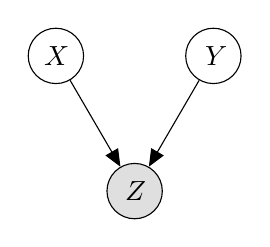
\begin{tikzpicture}
            \node[obs] (z) {$Z$};%
            \node[latent,above=of z,xshift=-1cm,fill] (x) {$X$}; %
            \node[latent,above=of z,xshift=1cm] (y) {$Y$}; %
            \edge {x,y} {z}
        \end{tikzpicture}
        }
        \DisplayProof
        \AxiomC{$X \perp Y \mid Z$}
        \RightLabel{\textsc{Fork}}
        \UnaryInfC{
        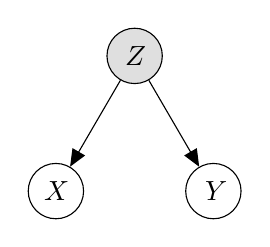
\begin{tikzpicture}
            \node[obs] (z) {$Z$};%
            \node[latent,below=of z,xshift=-1cm,fill] (x) {$X$}; %
            \node[latent,below=of z,xshift=1cm] (y) {$Y$}; %
            \edge {z} {x,y}
        \end{tikzpicture}
        }
        \DisplayProof
        \AxiomC{$X \perp Y \mid Z$}
        \RightLabel{\textsc{Chain}}
        \UnaryInfC{
        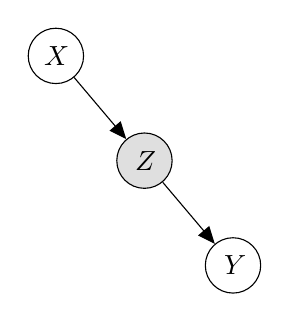
\begin{tikzpicture}
            \node[obs] (z) {$Z$};%
            \node[latent,above=of z,yshift=-11pt, xshift=-32pt,fill] (x) {$X$}; %
            \node[latent,below=of z,yshift=11pt, xshift=32pt] (y) {$Y$}; %
            \edge {x} {z}
            \edge {z} {y}
        \end{tikzpicture}
        }
    \end{prooftree}

    \noindent A Bayesian belief network (BN) is an acyclic DGM of the following form:
    \begin{equation*}
        P(x_1,\ldots,x_D)=\prod_{i=1}^D P(x_i \mid \texttt{parents}(x_i))
    \end{equation*}

    \noindent PGMs are very expressive, but even approximate inference on BNs is known to be NP-hard~\citep{dagum1993approximating}. We can faithfully represent a large class of PGMs and their corresponding distributions as probabilistic circuits (PCs)~\citep{choi2020probabilistic}, which are capable of exact inference in polynomial time and empirically tractable to calibrate using SGD or EM. PCs share many algebraic properties in common with PGMs and can propagate statistical estimators like variance and higher moments using simple algebraic rules. A PC is formed by taking recursive sums and products of univariate distributions~\cite{friesen2016sum}, as seen below:

    \begin{tabular}{cc}
        \hspace{-1.8cm}
        \begin{minipage}[c]{0.5\textwidth}
            \centering
            \begin{tabular}{l}
                $PC \rightarrow v \sim \mathcal{D}$ \\
                $PC \rightarrow PC \oplus PC$ \\
                $PC \rightarrow PC \otimes PC$
            \end{tabular}
        \end{minipage}
        &
        \begin{minipage}[c]{0.5\textwidth}
            \centering
            \digraph[scale=0.4]{spn1}{
                margin=0
                compound=true
                rankdir=LR
                node [shape=Mrecord,fontname="JetBrains Mono"]
                edge [fontsize=8,fontcolor=indigo]
                bgcolor=transparent
                nslimit=20

                g0 [label="{{μ|σ}|Normal|{<Out0>g0}}"]
                g1 [label="{{μ|σ}|Normal|{<Out0>g1}}"]
                g2 [label="{{μ|σ}|Normal|{<Out0>g2}}"]
                g3 [label="{{μ|σ}|Normal|{<Out0>g3}}"]

                f4 [label="{{<In0>g0|<In1>g1|<In2>g2}|Σ|{<Out0>f4}}"]
                f5 [label="{{<In0>f4|<In1>g3}|Π|{<Out0>f5}}"]

                g0:Out0 -> f4:In0
                g1:Out0 -> f4:In1
                g2:Out0 -> f4:In2
                g3:Out0 -> f5:In1
                f4:Out0 -> f5:In0


                out1 [style=invis,shape=point]
                out2 [style=invis,shape=point]

                f5 -> out1
            }
        \end{minipage}
    \end{tabular}

%    \noindent Given a BN, we can compile it to a SPN using the following procedure~\cite{butz2019sum}:
%
%    \begin{tabular}{cc}
%        \\
%        \hspace{-1cm}
%        \begin{minipage}[c]{0.5\textwidth}
%            \footnotesize
%        \begin{algorithm}
%            \begin{algorithmic}
%                \Procedure{Translate}{b: BN}: SPN
%                \State c $\leftarrow $\Call{VariableEliminate}{b}
%                \State s $\leftarrow $\Call{RedistributeParameters}{c}
%                \State s $\leftarrow $\Call{CompileMarginalized}{s}
%                \State \Return{\Call{Canonicalize}{s}}
%                \EndProcedure
%            \end{algorithmic}
%            \end{algorithm}
%        \end{minipage}
%        &
%        \hspace{-0.8cm}
%        \begin{minipage}[c]{0.52\textwidth}
%            \footnotesize
%    \begin{algorithm}
%        \begin{algorithmic}
%                \Procedure{Canonicalize}{s$_0$: SPN}: SPN
%                \State s$_1 \leftarrow$ \Call{AddTerminals}{s$_0$}
%                \State s$_1 \leftarrow$ \Call{MergeProducts}{s$_1$}
%                \State $\textbf{if } $s$_0 =$ s$_1$ \textbf{ then return } s$_1$
%                \State $\textbf{else return }$\Call{Canonicalize}{s$_1$}
%                \EndProcedure
%            \end{algorithmic}
%        \end{algorithm}
%    \end{minipage}
%    \end{tabular}



    \pagebreak\subsection{Knowledge is a graph}\label{subsec:kgs}

    \textit{Abduction} is the process of knowledge distillation: recognizing \textit{patterns} or \textit{motifs} in raw data, forming discrete \textit{categories} or \textit{types} of objects which share similar attributes, and adding edges representing abstract relations between types, such as composition, causation, or subsumption. The key idea is moving from the space of unstructured data to a structured domain containing abstract concepts and their relations. This domain is a graph.

    Knowledge graphs~\citep{hogan2020knowledge} are \textit{multi-relational graphs}, or \textit{hypergraphs} whose edges possess at least one type. Our work is primarily concerned with \textit{procedural knowledge}, or knowledge whose topology describes how to structure computation in order to achieve some desired task, although the technique we propose can also be applied to arbitrary directed, typed hypergraphs.

    The vertices in our graph represent \textit{functions} in some typed programming language and the edges represent their input and output types. Functions may be related by multiple types, and each type may relate multiple functions. Let $|\mathcal T|$ be the number of types in our system and $|\mathcal{F}|$ be the number of functions. We call our structure a \textit{type tensor}, $\mathbb{B}^{|\mathcal{F}|\times|\mathcal{T}|\times|\mathcal T|}$, also known as a \textit{logic table} or a \textit{data cube}. Consider the case where $|\mathcal F| = |\mathcal T| = 3$:

    \definecolor{R}{RGB}{202,65,55}
    \definecolor{G}{RGB}{151,216,56}
    \definecolor{B}{RGB}{0,0,0}
    \definecolor{W}{RGB}{255,255,255}
    \definecolor{X}{RGB}{65,65,65}

    \newcommand{\TikZRubikFaceLeft}[9]{\def\myarrayL{#1,#2,#3,#4,#5,#6,#7,#8,#9}}
    \newcommand{\TikZRubikFaceRight}[9]{\def\myarrayR{#1,#2,#3,#4,#5,#6,#7,#8,#9}}
    \newcommand{\TikZRubikFaceTop}[9]{\def\myarrayT{#1,#2,#3,#4,#5,#6,#7,#8,#9}}
    \newcommand{\BuildArray}{\foreach \X [count=\Y] in \myarrayL%
    {\ifnum\Y=1%
    \xdef\myarray{"\X"}%
    \else%
    \xdef\myarray{\myarray,"\X"}%
    \fi}%
    \foreach \X in \myarrayR%
    {\xdef\myarray{\myarray,"\X"}}%
    \foreach \X in \myarrayT%
    {\xdef\myarray{\myarray,"\X"}}%
    \xdef\myarray{{\myarray}}%
    }
    \TikZRubikFaceLeft
    {X}{W}{W}
    {W}{X}{X}
    {X}{W}{W}
    \TikZRubikFaceRight
    {W}{X}{W}
    {X}{W}{X}
    {W}{X}{W}
    \TikZRubikFaceTop
    {X}{W}{X}
    {W}{W}{X}
    {W}{X}{W}
    \BuildArray
    \pgfmathsetmacro\radius{0.1}
    \tdplotsetmaincoords{55}{135}

    \showcellnumberfalse


    \bgroup
    \def\arraystretch{1.2}
    \begin{table}[H]
        \centering
        \begin{tabular}{cc}
            \textbf{Typed Graph} & \textbf{Type Tensor} \\
            \begin{adjustbox}{minipage={.49\textwidth}, margin*=-0.5cm 0cm -0.5cm 0cm}
            \digraph[scale=0.5]{abcext3}{
            node[ fontname="CMU Classical Serif" fontsize=20 shape=Mrecord ];
            edge[ fontname="CMU Classical Serif" fontsize=18 ];
            rankdir=LR;
            len=3;

            f [ label="g"; ]
            a [ label="a"; ]
            c [ label="c"; ]
            d [ label="‖·‖" fontname="CMU Sans Serif" ]

%    a -> a [label="Σ₀"]
            f -> d [label="Ω"]
            d -> a [label="Ω"]
            d -> c [label="Ω"]
            }\hspace{-20pt}\digraph[scale=0.5]{abcext4}{
            node[ fontname="CMU Classical Serif" fontsize=20 shape=Mrecord ];
            edge[ fontname="CMU Classical Serif" fontsize=18 ];
            rankdir=LR;
            len=3;

            f [ label="g"; ]
            a [ label="a"; ]
            c [ label="c"; ]
            d [ label="‖·‖" fontname="CMU Sans Serif" ]

%    a -> a [label="Σ₀"]
            d -> f [label="ℤ"]
            a -> d [label="ℤ⁴"]
            c -> d [label="ℤ⁴"]
            } \end{adjustbox} & \begin{adjustbox}{minipage={.48\textwidth}}
            \begin{tikzpicture}
        \clip (-3,-2.5) rectangle (3,2.5);
        \begin{scope}[tdplot_main_coords]
            \filldraw [canvas is yz plane at x=1.5] (-1.5,-1.5) rectangle (1.5,1.5);
            \filldraw [canvas is xz plane at y=1.5] (-1.5,-1.5) rectangle (1.5,1.5);
            \filldraw [canvas is yx plane at z=1.5] (-1.5,-1.5) rectangle (1.5,1.5);
            \foreach \X [count=\XX starting from 0] in {-1.5,-0.5,0.5}{
            \foreach \Y [count=\YY starting from 0] in {-1.5,-0.5,0.5}{
            \pgfmathtruncatemacro{\Z}{\XX+3*(2-\YY)}
            \pgfmathsetmacro{\mycolor}{\myarray[\Z]}
            \draw [thick,canvas is yz plane at x=1.5,shift={(\X,\Y)},fill=\mycolor] (0.5,0) -- ({1-\radius},0) arc (-90:0:\radius) -- (1,{1-\radius}) arc (0:90:\radius) -- (\radius,1) arc (90:180:\radius) -- (0,\radius) arc (180:270:\radius) -- cycle;
            \ifshowcellnumber
            \node[canvas is yz plane at x=1.5,shift={(\X+0.5,\Y+0.5)}] {\Z};
            \fi
            \pgfmathtruncatemacro{\Z}{2-\XX+3*(2-\YY)+9}
            \pgfmathsetmacro{\mycolor}{\myarray[\Z]}
            \draw [thick,canvas is xz plane at y=1.5,shift={(\X,\Y)},fill=\mycolor] (0.5,0) -- ({1-\radius},0) arc (-90:0:\radius) -- (1,{1-\radius}) arc (0:90:\radius) -- (\radius,1) arc (90:180:\radius) -- (0,\radius) arc (180:270:\radius) -- cycle;
            \ifshowcellnumber
            \node[canvas is xz plane at y=1.5,shift={(\X+0.5,\Y+0.5)},xscale=-1] {\Z};
            \fi
            \pgfmathtruncatemacro{\Z}{2-\YY+3*\XX+18}
            \pgfmathsetmacro{\mycolor}{\myarray[\Z]}
            \draw [thick,canvas is yx plane at z=1.5,shift={(\X,\Y)},fill=\mycolor] (0.5,0) -- ({1-\radius},0) arc (-90:0:\radius) -- (1,{1-\radius}) arc (0:90:\radius) -- (\radius,1) arc (90:180:\radius) -- (0,\radius) arc (180:270:\radius) -- cycle;
            \ifshowcellnumber
            \node[canvas is yx plane at z=1.5,shift={(\X+0.5,\Y+0.5)},xscale=-1,rotate=-90] {\Z};
            \fi
            }
            }

            \draw [decorate,decoration={calligraphic brace,amplitude=10pt,mirror},yshift=0pt, line width=1.25pt]
            (3,0) -- (3,3) node [black,midway,xshift=-8pt, yshift=-14pt] {\footnotesize $\mathcal{T}$};
            \draw [decorate,decoration={calligraphic brace,amplitude=10pt},yshift=0pt, line width=1.25pt]
            (3,0) -- (0,-3) node [black,midway,xshift=-16pt, yshift=0pt] {\footnotesize $\mathcal{F}$};
            \draw [decorate,decoration={calligraphic brace,amplitude=10pt},yshift=0pt, line width=1.25pt]
            (0,-3) -- (-3,-3) node [black,midway,xshift=-8pt, yshift=14pt] {\footnotesize $\mathcal{T}$};
        \end{scope}
            \end{tikzpicture}
            \end{adjustbox}
        \end{tabular}
    \end{table}
    \egroup

    \vspace{-20pt}A type tensor indexed by a bijection $\mathcal{F} \times \mathcal{T} \times \mathcal{T} → \mathbb{N}^3$ is a type-level function $C[\![\cdot]\!] \subseteq \mathcal{F} \times \mathcal{T} → \mathcal{T}$ mapping a function $C: \mathcal{F}$ and type $T: \mathcal{T}$ to a set of reachable types $T^* \subseteq \mathcal{T}$, the congruence closure $C[\![T^*]\!] \equiv T^*$ of $T$ under $C$. Given a concrete type $S: \mathcal{T}$ and a one-hole context, $C[\![\cdot]\!]: ? → S$, synthesis in our type system consists of applying tensor contraction to compute the preimage of $S$ under $C$, $C^{-1}[\![S^*]\!]$. We leave this procedure for future work.

%    While subtyping, parametricity and higher-kinded types are possible to encode by considering higher-rank tensors, here we devote our attention to the simply-typed, rank-3 setting, in which every function maps a concrete type to a concrete type closed under composition. We adopt Chiang et al.'s named tensor notation~\cite{chaing2020named}. The typing rules for this procedure are defined below.
%
%    \begin{prooftree}
%        \AxiomC{$Γ ⊢ C[\![T]\!]: T → ?$}
%        \RightLabel{\textsc{Prop}}
%        \UnaryInfC{$Γ ⊢ C[\![T]\!]: T → C^{n = n+1}[\![S]\!]$}
%        \DisplayProof
%        \hskip 1.5em
%        \AxiomC{$Γ ⊢ C[\![\cdot]\!]: ? → T$}
%        \RightLabel{\textsc{Fill}}
%        \UnaryInfC{$Γ ⊢ C^{n = n+1}[\![T \in s^* \subseteq \mathcal{F}]\!]$}
%    \end{prooftree}
%
%    \noindent To increase the speed of type inference, we can precompute the congruence $C[\![\cdot]\!]$ and preimage closure $C^{-1}[\![\cdot]\!]$ so that $\textsc{Infer}$ and $\textsc{Fill}$ are both $\mathcal{O}(1)$. The type tensor simply enumerates paths between types in our type system, but does not tell us how likely a given path is to occur in an arbitrary program. To compute this probability, we need a stochastic transition matrix between functions, $\mathcal{F}\times\mathcal{F}$ representing the probability that some function is mapped to another. We plan to discuss this aspect in future work.

    \subsection{Algebraic graphs}\label{subsec:algebraic-graphs}

    The connection between algebra and graphs runs deep, unifying many seemingly disparate topics. A commutative monoid $(S, •, \circled{1})$ is a set $S$ with a binary operator $•: S \times S → S$ which has the following properties:

    \begin{prooftree}
        \bottomAlignProof
        \AxiomC{$a • (b • c)$}
        \UnaryInfC{$(a • b) • c$}
        \noLine
        \UnaryInfC{}
        \noLine
        \UnaryInfC{\textit{Associativity}}
        \DisplayProof
        \hskip 2.5em
        \bottomAlignProof
        \AxiomC{$a • \circled 1$}
        \UnaryInfC{$a$\vphantom{$()$}}
        \noLine
        \UnaryInfC{}
        \noLine
        \UnaryInfC{\textit{Neutrality}}
        \DisplayProof
        \hskip 2.5em
        \bottomAlignProof
        \AxiomC{$a • b$}
        \UnaryInfC{$b • a$\vphantom{$()$}}
        \noLine
        \UnaryInfC{}
        \noLine
        \UnaryInfC{\textit{Commutativity}}
    \end{prooftree}

    \noindent A semiring algebra, denoted $(S, \oplus, \otimes, \circled{0}, \circled{1})$, is a set together with two binary operators $\oplus, \otimes: S \times S → S$ such that $(S, \oplus, \circled{0})$ is a commutative monoid and $(S, \otimes, \circled{1})$ is a monoid. It has the following additional properties:

    \begin{prooftree}
        \bottomAlignProof
        \AxiomC{$a \otimes (b \oplus c)$}
        \UnaryInfC{$(a \otimes b) \oplus (a \otimes c)$}
        \noLine
        \UnaryInfC{}
        \AxiomC{$(a \oplus b) \otimes c$}
        \UnaryInfC{$(a \otimes c) \oplus (b \otimes c)$}
        \noLine
        \UnaryInfC{}
        \noLine
        \BinaryInfC{\textit{Distributivity}}
        \DisplayProof
        \hskip 2.5em
        \bottomAlignProof
        \AxiomC{$a \otimes \circled 0$}
        \UnaryInfC{$\circled 0$\vphantom{$()$}}
        \noLine
        \UnaryInfC{}
        \noLine
        \UnaryInfC{\textit{Annihilation}}
    \end{prooftree}

    \noindent Using iterated matrix multiplication on semirings, it is possible solve a wide variety of path problems. Known as \textit{propagation} or \textit{message passing}, this procedure consists of two steps: \textit{aggregate} and \textit{accumulate}. Let $\mathbf D_{st}$ denote some distance metric on a path between two vertices $s$ and $t$ in a graph. To obtain $\mathbf D_{st}$, one may run the following procedure on a desired path algebra:

    \begin{center}
        \begin{tabular}{lc|cr}
            $\mathbf{D}_{st} = \overbrace{\underset{P\in P_{st}^*}{\bigoplus}\underbrace{\underset{e\in P}{\bigotimes}W_{e}}_{\text{Aggregate}}}^{\text{Accumulate}}$ & & &
            \bgroup
            \def\arraystretch{1.2}
        \begin{tabular}{c|c{1cm}c{1cm}|c{1cm}c{1cm}|c}
            S                           & $\oplus$ & $\otimes$ & $\circled{0}$ & $\circled{1}$ & Path     \\\hline
            $\mathbb R \cup \{\infty\}$ & min      & +         &   $\infty$    &      0        & Shortest \\
            $\mathbb R \cup \{\infty\}$ & max      & +         &   $-\infty$   &      0        & Longest  \\
            $\mathbb R \cup \{\infty\}$ & max      & min       &       0       &   $\infty$    & Widest   \\
        \end{tabular}
            \egroup
        \end{tabular}
    \end{center}

    \noindent Many dynamic programming algorithms, including Bellman-Ford, Floyd-Warshall, Dijkstra, error, belief and expectation propagation, Markov chains, and others can all be neatly expressed as message passing with a semiring algebra. We refer the curious reader to explore~\cite{gondran2008graphs,baras2010path} for a more complete summary of the algebraic path problem and its many wonderful applications.

%    Suppose $\mathbf M$ is a positive matrix, such that $\mathbf M_{ij}$ is strictly positive. According to the Perron-Frobenius theorem, if $\mathbf M \in \mathcal T^{n \times n}$, then $\mathbf M$ has a unique largest eigenvalue $\lambda \in \mathcal T$ and dominant eigenvector $\mathbf{q} \in \mathcal T^{n}$. Assuming $\mathcal{T}$, $\lim_{i\rightarrow \infty} \mathbf{M}^i \mathbf{v} = c\mathbf{q}$ where $c$ is a constant.

%    $f(x, y) = \begin{bmatrix} \frac{cos(x+2y)}{x} & 0 \\ 0 & \frac{sin(x-2y)}{y} \end{bmatrix} * \begin{bmatrix}x\\y\end{bmatrix} = \begin{bmatrix}cos(x+2y)\\sin(x-2y)\end{bmatrix}$
%
%    \begin{tikzpicture}
%        \begin{axis}[
%            xmin = -4, xmax = 4,
%            ymin = -4, ymax = 4,
%            zmin = 0, zmax = 1,
%            axis equal image,
%            view = {0}{90},
%        ]
%            \addplot3[
%            quiver = {
%                u = {-x},
%                v = {y},
%            },
%            -stealth,
%            domain = -4:4,
%            domain y = -4:4,
%            ] {0};
%        \end{axis}
%    \end{tikzpicture}

    \pagebreak\section{From code to procedural knowledge}\label{sec:applications}

    \textit{Procedural knowledge} is knowledge designed or discovered to facilitate a process. Unlike \textit{relational knowledge} which may be bidirectional, procedural knowledge has a specific direction or goal. The methods presented in this literature review have broad applications to parsing and indexing procedural knowledge. Given a sequence of \textit{paths}, or \textit{traces} representing discrete steps in a goal-directed process with intermediate results, our research seeks to provide a mechanism for estimating procedural similarity, to synthesize or recommend semantically similar procedures under feasible reorderings. Specifically, our work focuses on the domain of \textit{programming} knowledge.

    Code shares many statistical properties in common with natural language and can be studied using natural language processing~\cite{hindle2012naturalness}. Unlike natural language, all syntactically-valid code has an unambiguous grammar. Furthermore, code primarily consists of \textit{functions} or \textit{procedures} intended to operate a machine. The underlying programming model may be relational, object-oriented or functional, but all mainstream programming languages support some form of procedure that accepts inputs and produces outputs.

    All procedures in a statically-typed programming language have a \textit{type signature}, for example, \texttt{getHomePhone: Person → PhoneNumber}. This represents a \textit{contract} between the procedure and its caller: if the procedure \texttt{getHomePhone} is called with a \texttt{Person}, it will return a \texttt{PhoneNumber}. All other inputs and outputs are forbidden by the type system. While often beneficial to consider more narrow definitions such as soundness or correctness, for procedural similarity these assumptions are unnecessary.

    Application programming interfaces (APIs) are a set of interfaces which describe available ways of structuring computation to achieve a set of related programming tasks. We call the graph of all possible ways to compose an API the \textit{API surface}. One traverses the API surface by composing accessible procedures in a \textit{call graph}. Thus, we can view the API as kind of a \textit{procedural knowledge base} representing common data transformations and how to compose them. In practice, how to achieve some desired goal is often far from obvious, requiring a large amount of documentation to explain.

    Many consumers of popular APIs publish code and documentation in open source repositories, a largely untapped source of knowledge for programming tools. Our work seeks to find ways of linking knowledge contained in open source repositories to help users locate examples and compose software applications. In the following section, we propose three applications of procedural pattern recognition for documentation alignment (\S~\ref{subsec:tracelink}), code search (\S~\ref{subsec:code-search}), program repair (\S\ref{subsec:code-search}), and eDSL generation (\S~\ref{subsec:code-search}).

    \subsection{Documentation alignment}\label{subsec:tracelink}

    Documentation is an indispensable resource for software developers learning to use a new API or programming language. Maintainers of popular software projects often publish web-based developer documents, typically in markup languages such as HTML or Markdown. These documents contain a mixture of natural language sentences, code snippets, and hyperlinks to related documents and source code files. All of these artifacts hold rich semantic information: the markup graph describes the text in relation to other entities in the document hierarchy, while the link graph describes relationships between relevant documents or artifacts in a software repository.

     Consider the typical workflow of a software developer who is seeking information about an unfamiliar API. To effectively locate relevant documentation, she must first copy a specific fragment of text (e.g. a function name, error message, or identifier) from a development environment into a search engine, providing relevant contextual information. The query must be descriptive enough to retrieve relevant documents with high probability, while omitting extraneous information (e.g. user-defined tokens) unlikely to occur outside the scope of the developer's personal environment or project.

    Prior work in information retrieval for software development investigated recommending API documentation~\cite{robillard2015recommending} and Q\&A content~\cite{treude2016augmenting} to developers. Similar work in natural language processing has studied the relationship between comments and source code entities~\cite{iyer2018mapping, panthaplackel2020associating} strictly within source code. Examples of cross-domain entity linking in the source-to-doc (S2D) and doc-to-source (D2S) setting are scarce, however these results indicate alignment between natural language and software artifacts may be feasible.

    Our work seeks to facilitate procedural knowledge discovery by enriching lexical queries with semantic information extracted from a programming environment, and prioritizing semantically relevant software artifacts among a set of matching search results. Broadly, the tools we have proposed in this literature review can be used to study both source code and procedural knowledge graphs, however due to the paucity of cross-domain entity links between code and natural language artifacts, reasoning about cross-domain relations will require developing new approaches to feature engineering, unsupervised learning and entity alignment in the low-data regime.

    Such an application, if successful, would allow developers to more quickly and easily locate semantically or contextually relevant code samples in API documentation and open source repositories. The same tools could also help authors maintain a consistent set of API documentation and usage examples across a large codebase, a persistent obstacle when evolving any API.

    \pagebreak\subsection{Code search}\label{subsec:code-search}

    Given a learned similarity metric between procedures, one straightforward application is code search. Prior work in this area has explored type-directed~\cite{james2020digging}, learning-based~\cite{gu2018deep} and semantic search~\cite{premtoon2020semantic} techniques. These techniques all use a fixed, or synthetic ordering over search results. For a given hole context, there are often many valid completions within an API or codebase. Given a corpus of procedures in their surrounding typing environment, is it possible to estimate a probability distribution on a shared embedding between contexts and results, and measure the likelihood that a given search result occurs in an empty location? This requires:

    \begin{enumerate}
        \item Efficiently searching a corpus for a well-typed pattern
        \item Ranking the matching search results by semantic alignment
        \item Incorporating information into user's context (e.g. variable renaming)
    \end{enumerate}

    Given a cursor and the surrounding context (e.g. in an IDE or editor), such a tool would need to search a database for the most similar contexts, extract common snippets to estimate their \textit{concordance} or \textit{agreement} with the surrounding code context, then adapt the foreign code snippet into to the user's context. External contexts including public code samples or API-documentation (e.g. fixes or repairs for compiler error messages) could help the user to complete some unfinished piece of code. Some open research questions include:

    \begin{enumerate}
        \item \textbf{Semantic segmentation}: How do we slice or truncate context?
        \item \textbf{Graph search}: What kernel be used for fast subgraph detection?
        \item \textbf{Context ranking}: What features to use to best measure similarity?
        \item \textbf{Refactoring}: How to integrate a selected result into the user's code?
    \end{enumerate}

    The proposed method presents an interesting engineering challenge. To work for code completion, it would need to have relatively low latency for a pleasant user experience. While the model could be trained on a large corpus offline, the contextual embedding would need to be periodically recomputed as the surrounding typing environment changes in the editor. Furthermore, the search and retrieval speed would need keystroke latency to be effective.

    \pagebreak\subsection{Program synthesis}\label{subsec:synthesis}

    In this proposal, we have seen a number of procedures for generating, or synthesizing a short procedure from a space of valid procedures. Various approaches are presented for determining the equivalence of valid procedures and sampling from a constrained space of representable functions to produce a higher-order probabilistic function, satisfying a set of constraints.

    Our initial approach described in~\S\ref{subsec:kgs}, simply enumerates paths between types in our type system, but does not tell us how likely a given path is to occur in a codebase. To compute this probability, we need a stochastic transition matrix between functions, $\mathcal{F}\times\mathcal{F}$ representing the probability that some function is to be composed with another. Given a grammar and type system, we would like a way of sampling novel programs according to the distribution of programs which occur in some codebase.

    \subsection{DSL generation}\label{subsec:gen}

    Most knowledge starts with pen on paper. It is generally possible for developers to translate well-structured pseudocode into code. However, there are many valid translations -- the same algorithm implemented in the same language by different authors is seldom written the same way. Instead of translating these ideas from scratch, it may be possible to encode just a few axioms and enough knowledge to derive a family of algorithms, reusing existing optimizations written by other developers and selecting the most appropriate procedure for computing a desired quantity, e.g. using a sufficiently expressive logic system, and a database of simple facts and relations.

    Knowledge systems or \textit{ontologies} are a collection of related facts designed or discovered by human beings. For example, we can treat mathematical knowledge as a kind of symbolic rewrite system. This has been successfully operationalized in Theano~\citep{bergstra2010theano} and other DSLs. It is possible to view constructive mathematics libraries like Metamath~\citep{megill2006metamath}, Rubi~\citep{rich2009knowledge}, Arend, KMath~\citep{nozik2019kotlin} and Kotlin$\nabla$~\citep{considine2019kotlingrad} as also working towards this high-level goal.

    In knowledge engineering, approximate equality is known as entity \textit{alignment} or \textit{matching}. With an approximate matching algorithm, we could accurately detect near-duplicates in a large codebase, find similar documentation snippets, retrieve contextually or semantically relevant code samples to assist developers writing unfamiliar code, and search for bugs in code or fixes from an external knowledge base to repair them. All of these tasks require some notion of semantic similarity between procedures.

    \pagebreak \section{Acknowledgements}

    The author wishes to thank his advisor Jin Guo, Xujie Si and Fuyuan Lyu, for providing several helpful comments on this proposal and Torsten Scholak, David Yu-Tung Hui, Disha Shrivastava, Jordi Armengol-Estap\'e, Matt Rice, Dave Keenan, and John Tromp for various miscellaneous feedback.

    \bibliography{exam_proposal}
    \bibliographystyle{plain}
\end{document}